\documentclass[tikz]{standalone}
\usepackage{amssymb,amsmath,mathtools}

\usetikzlibrary{fit}
\usetikzlibrary{shapes,arrows}
\usetikzlibrary {shapes.misc} 
\usetikzlibrary{arrows.meta}
\usetikzlibrary{calc,positioning}
\usetikzlibrary{patterns,decorations.pathmorphing,decorations.markings}

\begin{document}

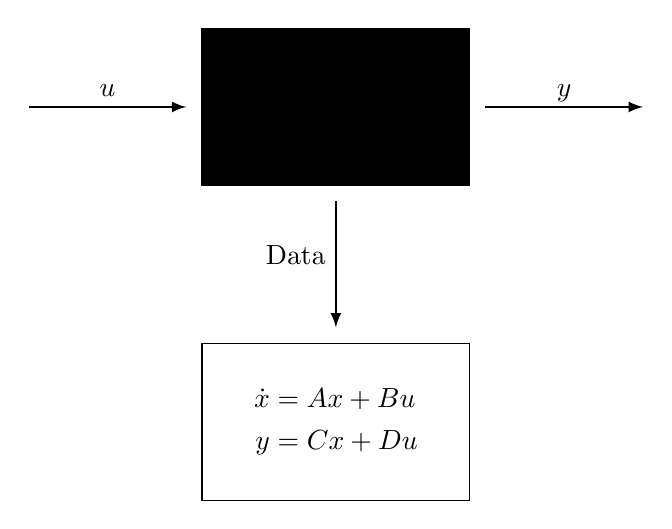
\begin{tikzpicture}[scale=2]% coordinates%\begin{}[]%\addplot coordinates {};%\end{}%\end{}
    \draw[fill=black,color=black] (1.1,4.5) rectangle (2.8,5.5);
    \draw[thick, -latex] (0,5) -- node[above] {$u$} (1,5);
    % \node at (1.95,5) {\textcolor{white}{\Huge$\Sigma$}};
    \draw[thick, -latex] (2.9,5) -- node[above] {\smash{$y$}} (3.9,5);
    
    \draw[thick, -latex] (1.95,4.4) -- node[left] {\smash{Data}} (1.95,3.6);
    
    \draw[color=black] (1.1,2.5) rectangle (2.8,3.5);
    % \node at (1.95,3) {\Huge$\Sigma
    % % _{\phantom{\mathrm{pH}}}
    % $};
    \node at (1.95,3) {
        $\begin{aligned}
            \dot{x} &= Ax + Bu\\
            y &= Cx + Du				
        \end{aligned}$
    };
        
\end{tikzpicture}

\end{document}